\documentclass[11pt]{article}

\usepackage{a4wide}
\usepackage{amsmath,amssymb}
\usepackage[english]{babel}
\usepackage{enumitem}
\usepackage{float}
\usepackage{graphicx}
\usepackage[utf8]{inputenc}
\usepackage{listings}
\usepackage{multicol}
\usepackage{tikz}

%========== DEFINITIONS & MACROS ==========%

\definecolor{comment}{rgb}		{0.38, 0.62, 0.38}
\definecolor{keyword}{rgb}		{0.10, 0.10, 0.81}
\definecolor{identifier}{rgb}	{0.00, 0.00, 0.00}
\definecolor{string}{rgb}		{0.50, 0.50, 0.50}

\newcommand{\secref}[1]{see section \ref{#1} on page \pageref{#1}}
\newcommand{\appref}[1]{see appendix \ref{#1} on page \pageref{#1}}
\newcommand{\txtref}[2][]{see {\it #1} \ref{#2} on page \pageref{#2}}
\newcommand{\code}[1]{{\tt #1}}
\newcommand{\file}[1]{{\tt #1}}
\newcommand{\imp}{\rightarrow}
\newcommand{\norm}[1]{\lVert#1\rVert}
\newcommand{\unit}[1]{\frac{#1}{\norm{#1}}}
\newcommand{\mat}[1]{\text{\bf #1}}

% usage: \codefig{label}{file}{firstline}{lastline}{description}
\newcommand{\codefig}[5]
{
\begin{figure}[H]
    \lstinputlisting[firstnumber=#3,firstline=#3,lastline=#4]{../../src/#2}
    \caption{#5}
    \label{code:#1}
\end{figure}
}

\setdescription{leftmargin=\parindent, labelindent=\parindent}

\lstset
{
    language=C++,
	% general settings
	numbers=left,
	frame=single,
	basicstyle=\footnotesize\ttfamily,
	tabsize=2,
	breaklines=true,
	% syntax highlighting
	commentstyle=\color{comment},
	keywordstyle=\color{keyword},
	identifierstyle=\color{identifier},
	stringstyle=\color{string},
}


\title
{
    {\Large Individual Assignment 5} \\
    Introduction to Computer Graphics
}

\author
{
    Casper B. Hansen \\
    University of Copenhagen \\
    Department of Computer Science \\
    {\tt fvx507@alumni.ku.dk}
}

\date{last revision \today}

\begin{document}

\clearpage\maketitle\vspace{1in}
\begin{multicols}{2}
    \begin{abstract}
        We will discuss the concept of Bezier curves and how they can be
        described in mathematical form. A discussion of how the geometry
        vector and basis matrix affects the behaviour of the Bezier curve, and
        lastly we will discuss the of three different implementation
        techniques.
        
        The reader is not expected to have any prior knowledge of the material
        presented. For the code the reader is expected to have some basic
        understanding of linear algebra and the C++ language.
    \end{abstract}
    \vfill\columnbreak\tableofcontents\vfill
\end{multicols}
\thispagestyle{empty}\newpage

\section{Theory}
The general form of a parametric curve is a vector function. That is, a scalar
{\it parameter} $t \in \mathbb{R}$ is given as the argument of the vector
function, which maps it to a vector $v \in \mathbb{R}^n$.
\begin{align}
    f : \mathbb{R} \imp \mathbb{R}^n
\end{align}
We can rewrite this in 3-dimensional vector form, as a polynomial of degree 3 in 3
dimensions.
\begin{align}
    f(t) &=
    \begin{bmatrix}
        x(t) \\
        y(t) \\
        z(t)
    \end{bmatrix}
    =
    \begin{bmatrix}
        a_x t^3 + b_x t^2 + c_x t + d_x \\
        a_y t^3 + b_y t^2 + c_y t + d_y \\
        a_z t^3 + b_z t^2 + c_z t + d_z
    \end{bmatrix}
    \quad
    0 \leq t \leq 1
\end{align}
For which the coordinate functions $x(t)$, $y(t)$ and $z(t)$ are regular
polynomials of degree 3.

\subsection{Coefficient Matrix}
Expanding this further, we can rewrite it in matrix form.
\begin{align}
    f(t) &=
    \begin{bmatrix}
        x(t) \\
        y(t) \\
        z(t)
    \end{bmatrix}
    =
    \begin{bmatrix}
        a_x + b_x + c_x + d_x \\
        a_y + b_y + c_y + d_y \\
        a_z + b_z + c_z + d_z
    \end{bmatrix}
    \begin{bmatrix}
        t^3 \\
        t^2 \\
        t   \\
        1
    \end{bmatrix}
    \quad
    0 \leq t \leq 1
\end{align}
This matrix is what we called the {\it coefficient matrix}, and we will denote
it in vector form as $\mat{C}$. We then have that $f(t) = \mat{C}t$.

\subsection{Geometry and Basis Matrices}
Since the $\mat{C}$ gives us little information about the shape of the curve,
we will expand $\mat{C}$ and write it as the product of two matrices; a {\it
geometry matrix} which we will denote as $\mat{G}$ and a {\it basis matrix}
which we will denote $\mat{M}$.

The geometry matrix contains information about the curve. That is, each column
vector of the geometry matrix describes the curves control points. Since all
information about the curve is contained within the geometry matrix, then the
basis matrix simply needs to transform the geometry matrix into $\mat{C}$,
making the basis matrix constant. The basis matrix determines the type of the
curve (i.e. Bezier, Hermitian, etc.).

Since the basis matrix is constant, let us define it. A curves points are
given by $f_H(t) = G_H M_H \begin{bmatrix}t^3 & t^2 & t & 1\end{bmatrix}^T$,
and its tangents are given by $f'_H(t) = G_H M_H \begin{bmatrix}3t^2 & 2^t & 1
& 0\end{bmatrix}^T$. We then have that
\begin{align}
    f_H(0) = G_1 = G_H M_H
    \begin{bmatrix}
        0 \\ 0 \\ 0 \\ 1
    \end{bmatrix}
    \quad
    \text{and}
    \quad
    f_H(1) = G_2 = G_H M_H
    \begin{bmatrix}
        1 \\ 1 \\ 1 \\ 1
    \end{bmatrix}
    \\
    f'_H(0) = G_3 = G_H M_H
    \begin{bmatrix}
        0 \\ 0 \\ 1 \\ 0
    \end{bmatrix}
    \quad
    \text{and}
    \quad
    f'_H(1) = G_4 = G_H M_H
    \begin{bmatrix}
        3 \\ 2 \\ 1 \\ 0
    \end{bmatrix}
\end{align}
And thus $M_H$ is given by the aboves inverse.
\begin{align}
    M_H &=
    \begin{bmatrix}
        1 & 0 & -3 &  0 \\
        0 & 0 &  3 &  0 \\
        0 & 0 &  0 & -3 \\
        0 & 1 &  0 &  3
    \end{bmatrix}^{-1}
    =
    \begin{bmatrix}
         2 & -3 & 0 & 1 \\
        -2 &  3 & 0 & 0 \\
         1 & -2 & 0 & 0 \\
         1 & -1 & 1 & 0
    \end{bmatrix}
\end{align}
This defines the basis matrix of Hermitian curves $M_H$. We can use a relation
between the Hermitian basis matrix to produce the Bezier basis matrix $M_B$ by
recognizing that $\begin{bmatrix}G_1 & G_2 & G_3 & G_4\end{bmatrix}_H =
\begin{bmatrix}G_1 & G_4 & 3(G_2 - G_1) & 3(G_4 - G_3)\end{bmatrix}_B$, giving
us the following basis conversion matrix.
\begin{align}
    G_H &= \begin{bmatrix}G_1 & G_2 & G_3 & G_4\end{bmatrix}_B
    \begin{bmatrix}
        1 & 0 & -3 &  0 \\
        0 & 0 &  3 &  0 \\
        0 & 0 &  0 & -3 \\
        0 & 1 &  0 &  3
    \end{bmatrix}_{B \imp H}
\end{align}
By this, we see that $G_H = G_B M_{B \imp H}$, and following through on this
we have that $f(t) = G_H M_H t = (G_B M_{B \imp H}) M_H t = G_B (M_{B \imp H}
M_H) t$. From this, we see that
\begin{align}
    M_B = M_{B \imp H} M_H =
    \begin{bmatrix}
        1 & 0 & -3 &  0 \\
        0 & 0 &  3 &  0 \\
        0 & 0 &  0 & -3 \\
        0 & 1 &  0 &  3
    \end{bmatrix}
    \begin{bmatrix}
         2 & -3 & 0 & 1 \\
        -2 &  3 & 0 & 0 \\
         1 & -2 & 0 & 0 \\
         1 & -1 & 1 & 0
    \end{bmatrix}
    =
    \begin{bmatrix}
         1 &  3 & -3 & 1 \\
         3 & -6 &  3 & 0 \\
        -3 &  3 &  0 & 0 \\
         1 &  0 &  0 & 0
    \end{bmatrix}
\end{align}
And thus, we have defined the basis matrix of Bezier curves. By inspection, we
can see that the basis matrix of Bezier curves creates a weighted sum of the
control points at the parameter $t$ --- in essence, the point on a Bezier
curve is pulled in all control point directions and is put in place by the
weight given for each control point at a given $t$.

This abstraction from $\mat{C}$ allows for easy interpretation and
modification of the curve geometry and how it is being transformed.

\newpage
\section{Implementation}
All of the algorithms are handled by the same \code{draw} method in the
\code{BezierVec4} class. Therefore, we declare the common elements at the head
of the function, including some helper macros to shorten the formulae.

\codefig{sampled}{BezierVec4.cpp}{60}{68}
{Code excerpt showing the common declarations and helper macros.}

\subsection{Sampled Curve}
The most computationally expensive way of computing a Bezier curve we will
look at is by way of {\it sampling}. We simply calculate each and every point
of the segments using the regular polynomial functions, as can be seen on
lines 79--82.

\codefig{sampled}{BezierVec4.cpp}{77}{89}
{Code excerpt showing the sampled curve algorithm.}

This method is not considered to be efficient in any way, but it is very
simple.

\begin{figure}[H]
    \center
    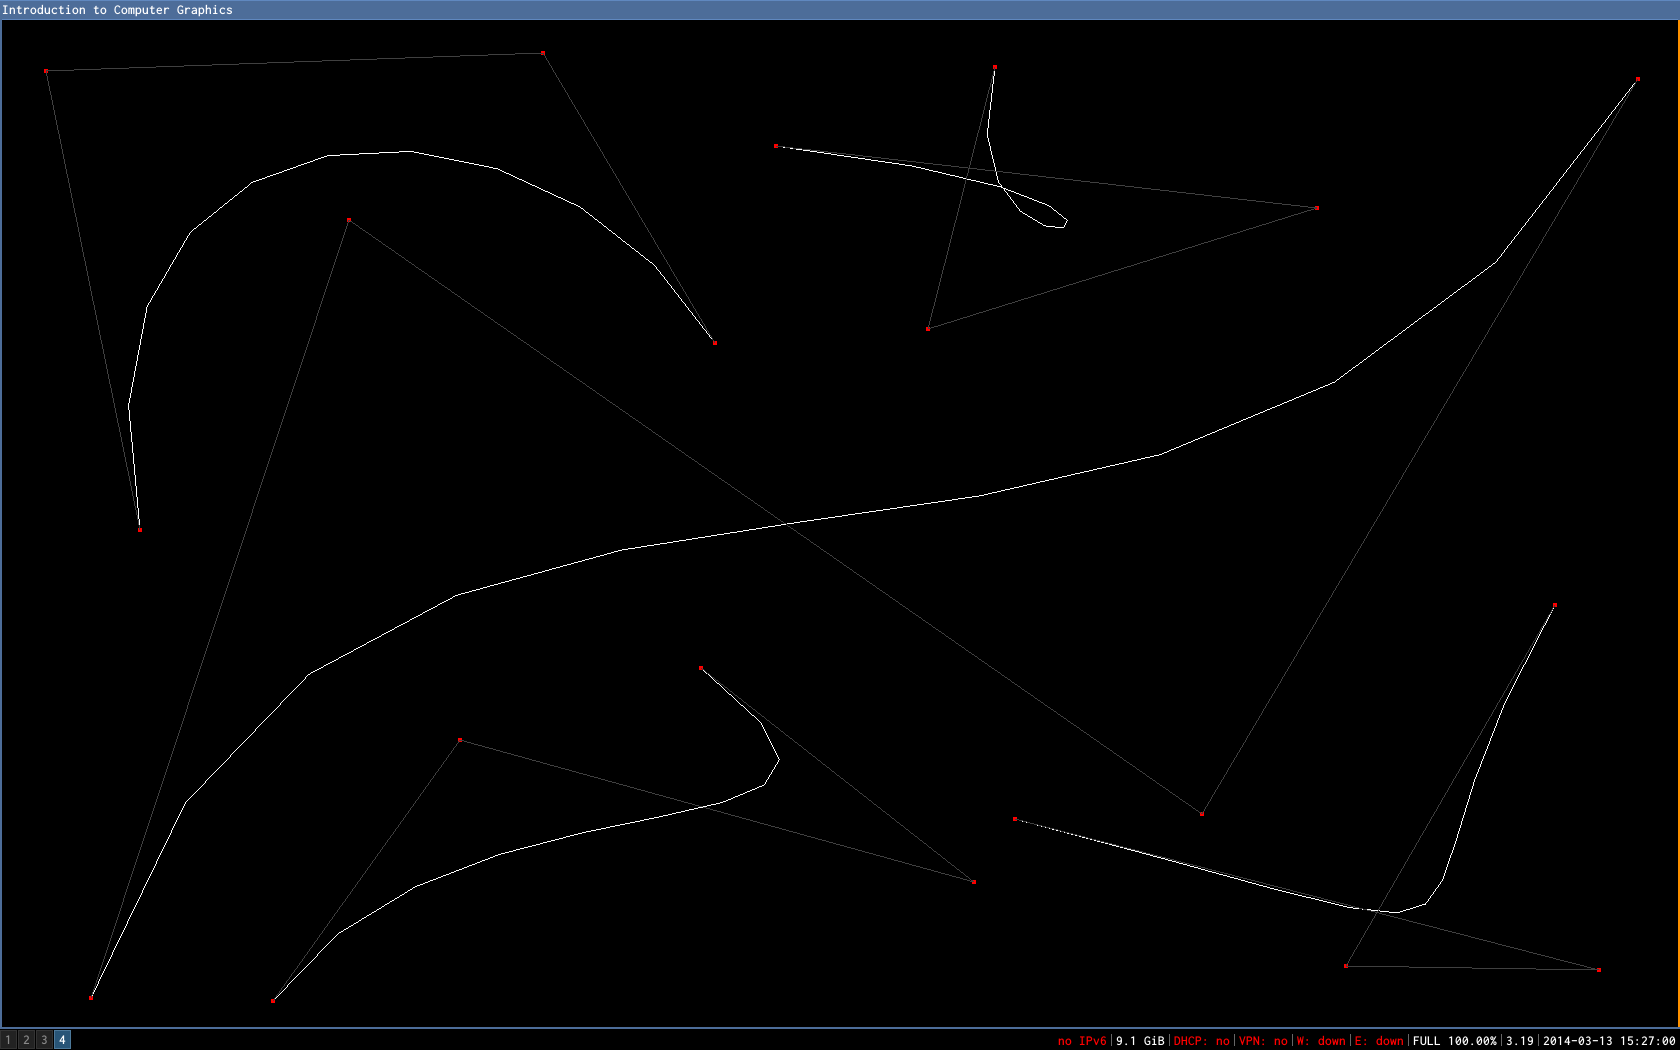
\includegraphics[scale=0.25]{figures/test-sampled.png}
    \caption{A screenshot showing sampled Bezier curves.}
    \label{fig:test-sampled}
\end{figure}

The above screenshot shows the how the sampled Bezier curve implementation
looks with 10 segments.

\subsection{Forward Difference}
This method is a lot more efficient than sampling discussed previously. It
using a lot of pre-calculation to reduce overhead and minimizes
computationally expensive operations.

Consider the polynomial coordinate function $f(t) = at^3 + bt^2 + ct + d$. We
want to calculate, from the starting point, the next point at an offset into
the curve of $\Delta t = \delta$.

We know that $\Delta f(t) = f(t + \delta) - f(t)$ and $f(t + \delta) = f(t) +
\Delta f(t)$, so we have that $f_{n+1} = f_n + \Delta f_n$. Substituting this
into the polynomial equation and reducing the expression, we have that
\begin{align}
    \Delta f(t) = 3a\Delta t^2 + (3a\Delta^2 + 2b\Delta)t + a\Delta^3 + b\Delta^2 + c\Delta
\end{align}
In which the highest order term is $3a\Delta t^2$, making it a polynomial of
degree 2. So, the original polynomial degree was decreased by one. Repeating
this procedure until we reach a constant expression yields
\begin{align}
    \Delta f(t)   &= 3a\Delta t^2 + (3a\Delta^2 + 2b\Delta)t + a\Delta^3 + b\Delta^2 + c\Delta \\
    \Delta^2 f(t) &= 6 a \Delta^2 t + 6 a \Delta^3 + 2 b \Delta^2 \\
    \Delta^3 f(t) &= 6 a \Delta^3
\end{align}
This is what is done on lines 101--110. Note also, that for this we have to
use the geometry vectors, which are calculated as discussed earlier on lines
95--99.

Now that we have the delta points, we can use them to incrementally calculate
the next point in the Bezier curve. The advancement is dependent on $\Delta$,
which we define as $\Delta = \frac{1}{n}$, where $n$ is the number of curve
segments. In looking at the differences across the delta points we find that
the initialization is then
\begin{align}
    \begin{bmatrix}
        f(0) \\
        \Delta f(0) \\
        \Delta^2 f(0) \\
        \Delta^3 f(0)
    \end{bmatrix}
    &=
    \begin{bmatrix}
        d \\
        a \Delta^3 + b \Delta^2 + c \Delta \\
        a \Delta^3 + 2 b \Delta^2 \\
        6 a \Delta^3
    \end{bmatrix}
\end{align}
as adding $\Delta^n f$ and $\Delta^{n-1} f$ produces the advanced $\Delta^n f$
for the following point. Thus, we simply have to update these accordingly,
while we render each point. This is done on lines 112--125.

\codefig{forward-diff}{BezierVec4.cpp}{95}{125}
{Code excerpt showing the forward difference algorithm.}

Note that on line 111 the condition of $t$ is in the interval
$[0; 1 - \frac{1}{n}]$. If we were to allow $t$ to reach $1$ in this loop, we
would go one curve segment beyond the last control point. This is side effect
of a poorly thought out loop invariant.

\begin{figure}[H]
    \center
    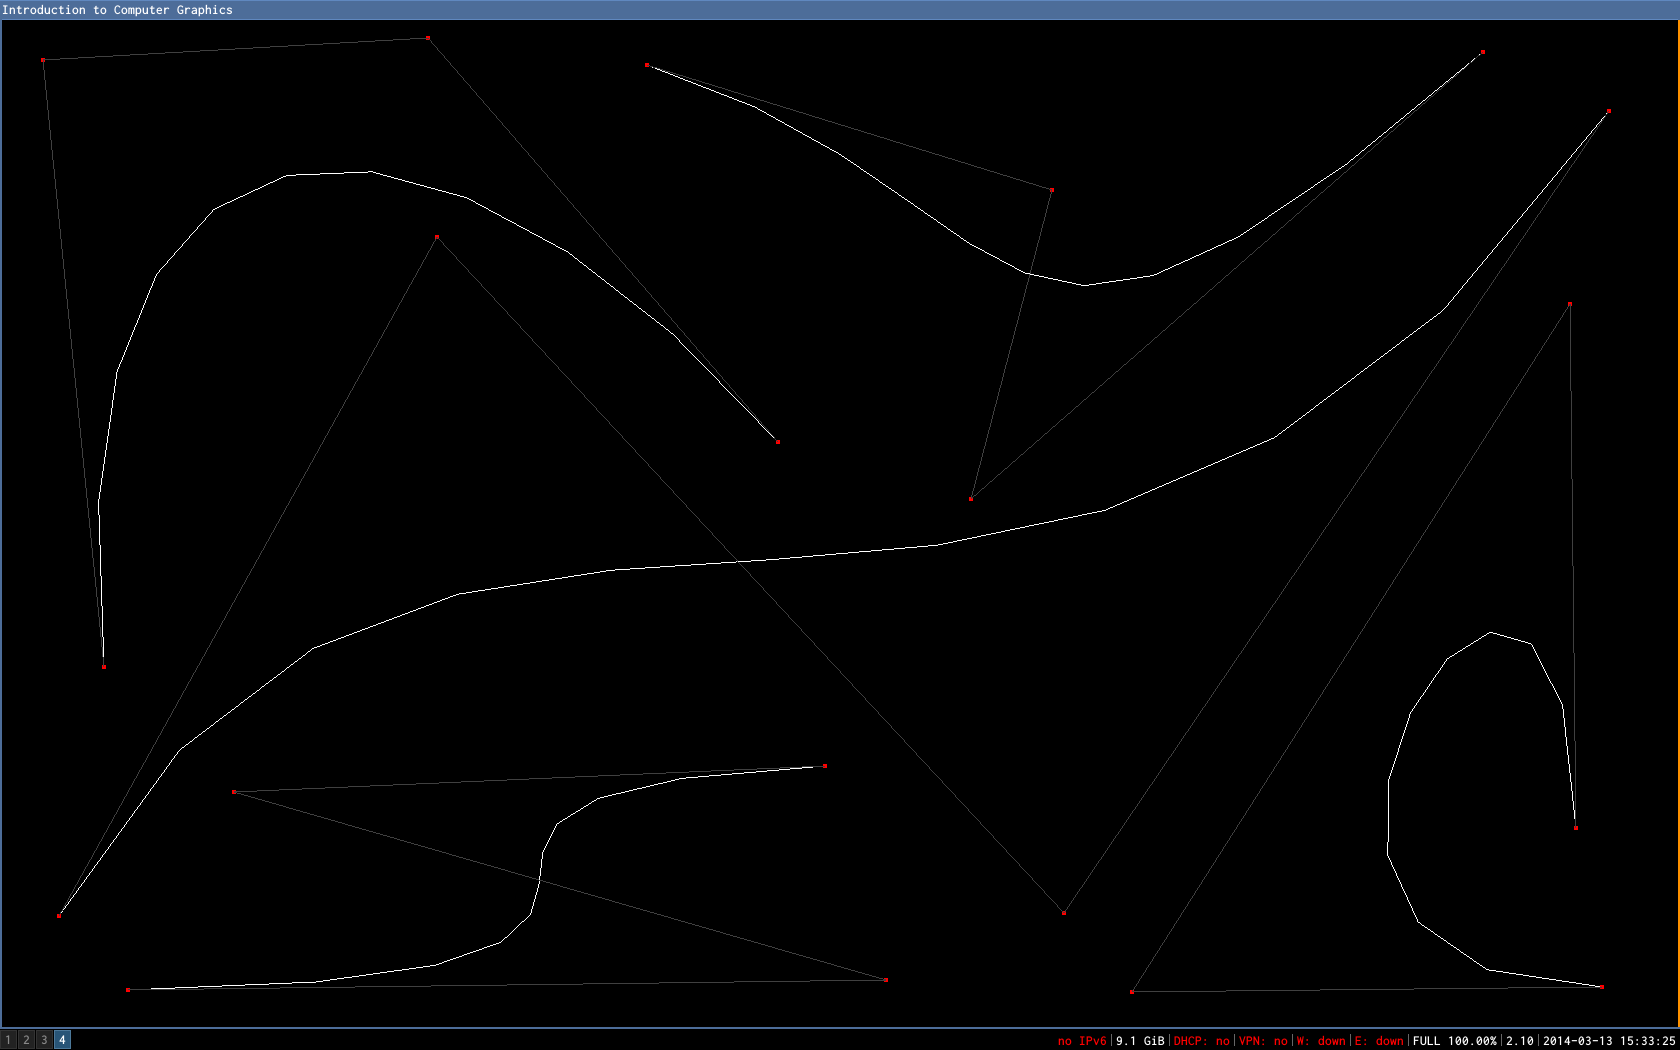
\includegraphics[scale=0.25]{figures/test-forward-diff.png}
    \caption{A screenshot showing forward differencing Bezier curves.}
    \label{fig:test-forward-diff}
\end{figure}

The above screenshot shows the how the forward difference Bezier curve
implementation looks with 10 segments.

\subsection{Subdivision}
The algorithm with the highest quality, however, is the subdivision algorithm.
It generates approximation points along the curve and in doing so it decreases
the distance from the approximation to the actual curve. Once an decent
distance is achieved it considers the points generated to be acceptable.

We consider a Bezier curve with control points $G_1$, $G_2$, $G_3$ and $G_4$.
Let $H$ be the midway point between $G_2$ and $G_3$, and let $L_2$ be the
midway point between $G_1$ and $G_2$, and let $R_2$ be the midway point
between $G_3$ and $G_4$. Further, let $L_3$ and $R_3$ be the midway points
between $H$ and $L_2$, and $H$ and $R_2$, respectively. Finally, let $L_1 =
G_1$ and $R_1 = G_4$, and let $L_4 = R_4$ be the midway point between $L_3$
and $R_3$.

We then have the following formulae at our disposal
\begin{align}
    H &= (G_2 + G_3) / 2
\end{align}
\vspace{-0.75in}
\begin{multicols*}{2}
    \begin{align}
        L_1 &= G_1 \\
        L_2 &= (G_1 + G_2) / 2 \\
        L_3 &= (H + L_2) / 2 \\
        L_4 &= (L_3 + R_3) / 2
    \end{align}
    \vfill\columnbreak
    \begin{align}
        R_1 &= G_4 \\
        R_2 &= (G_3 + G_4) / 2 \\
        R_3 &= (H + L_2) / 2 \\
        R_4 &= (L_3 + R_3) / 2
    \end{align}
\end{multicols*}
These expressions constitute newly generated points on of the curve. In the
code these are defined on lines 185--192.

Now, we have to determine whether or not these points are close enough
approximations of the curve. This is done by the so-called {\it flatness test}
for which we will need to determine the distance function.
\begin{align}
    d(x) &=
    \left|(x - G_1) - \left[(x - G_1) \cdot \frac{G_4 - G_1}{\lvert G_4 - G_1 \rvert}\right] \frac{G_4 - G_1}{\lvert G_4 - G_1 \rvert} \right|
\end{align}
We use this to determine how far away the points $G_2$ and $G_3$ are on lines
162--168. The farthest point is then used for comparison with the $\epsilon$
on line 170. If the point exceeds the $\epsilon$ we recurse with the $L$ and
$R$ points generated on lines 194--195, otherwise we simply draw the segments
on lines 172--181.

\codefig{sampled}{BezierVec4.cpp}{162}{196}
{Code excerpt showing the subdivision algorithm.}

\begin{figure}[H]
    \center
    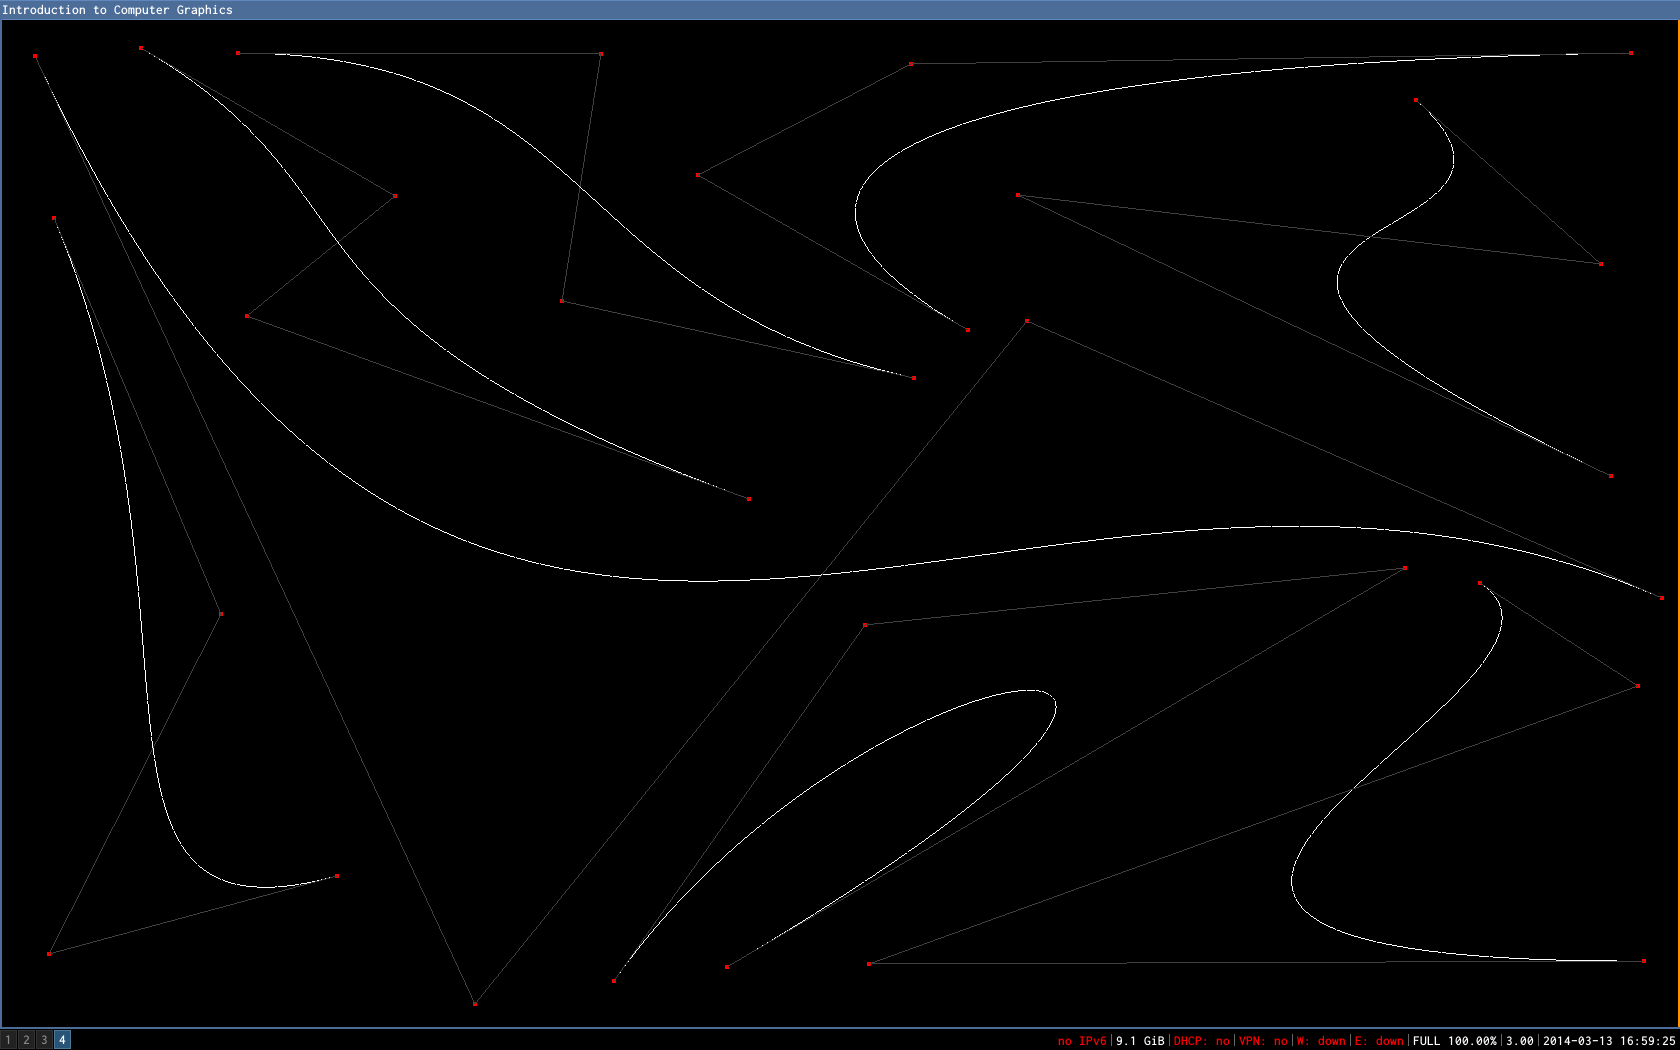
\includegraphics[scale=0.25]{figures/test-subdivision.png}
    \caption{A screenshot showing subdivision of Bezier curves.}
    \label{fig:test-subdivision}
\end{figure}

\end{document}

